\documentclass[11pt]{article}
\usepackage{setspace}
\setstretch{1}
\usepackage{amsmath,amssymb, amsthm}
\usepackage{graphicx}
\usepackage{bm}
\usepackage[hang, flushmargin]{footmisc}
\usepackage[colorlinks=true]{hyperref}
\usepackage[nameinlink]{cleveref}
\usepackage{footnotebackref}
\usepackage{url}
\usepackage{listings}
\usepackage[most]{tcolorbox}
\usepackage{inconsolata}
\usepackage[papersize={8.5in,11in}, margin=1in]{geometry}
\usepackage{float}
\usepackage{caption}
\usepackage{esint}
\usepackage{url}
\usepackage{enumitem}
\usepackage{subfig}
\usepackage{wasysym}
\newcommand{\ilc}{\texttt}
\usepackage{etoolbox}
\usepackage{algorithm}
\usepackage{changepage}
% \usepackage{algorithmic}
\usepackage[noend]{algpseudocode}
\usepackage{tikz}
\usetikzlibrary{matrix,positioning,arrows.meta,arrows}
\patchcmd{\thebibliography}{\section*{\refname}}{}{}{}
% \PassOptionsToPackage{hyphens}{url}\usepackage{hyperref}

\providecommand{\myceil}[1]{\left \lceil #1 \right \rceil }
\providecommand{\myfloor}[1]{\left \lfloor #1 \right \rfloor }


\begin{document}



\title{\textbf{CSDS 455: Homework 8}}

\author{Shaochen (Henry) ZHONG, \ilc{sxz517}}
\date{Due and submitted on 09/21/2020 \\ Fall 2020, Dr. Connamacher}
\maketitle

\section*{Problem 1}
\textbf{W.T.S $\lambda(G) \leq \delta(G)$:} Let $v \in V(G)$ with $\delta(v) = \delta(G)$, this suggest by removing every edges connected to $v$ we can clearly have disconncted part (the isolated $v$). This suggest $\lambda(G) = \delta(G)$.

However it is possible to have $\delta(V) < \delta(G)$, in the below example we have $\delta(G) = 2$, however by simply remove the $AB$ edge we can have a disconncted graph. Thus, $\lambda(G) \leq \delta(G)$.

\begin{figure}[H]
    \centering
    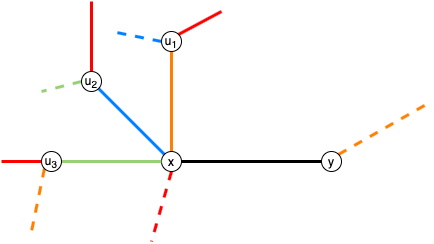
\includegraphics[width=0.45\linewidth]{{fig/fig_p1_1.png}}
    \label{fig:1_1}
\end{figure}

\textbf{W.T.S $\kappa(G) \leq \lambda(G)$:}

We know that we may have $\kappa(G) = \lambda(G)$ in a sense of $P2$ (two-vertex line), where to break it into a disconncted graph we will have $\kappa(G) = \lambda(G)$. However, it is possible to have $\kappa(G) < \lambda(G)$. In the below example we will need to remove edge $AC$ and $CB$ to make $G$ disconncted, which suggest $\lambda(G) = 2$; but we can also make $G$ disconncted by removing $C$, which yields a $\kappa(G) = 1$. Thus, we have $\kappa(G) \leq \lambda(G)$.\newline

\begin{figure}[H]
    \centering
    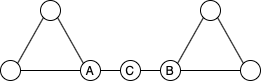
\includegraphics[width=0.45\linewidth]{{fig/fig_p1_2.png}}
    \label{fig:1_2}
\end{figure}

Combine with the above to findings, we have $\kappa(G) \leq \lambda(G) \leq \delta(G)$.

\section*{Problem 2}
\section*{Problem 3}
\section*{Problem 4}








% \section{References}
%
% \nocite{*}
% \raggedright
% \bibliography{references.bib}
% \bibliographystyle{plain}


\end{document}